\document[./main_hagedorn.tex]{subfiles}
\usepackage{amsmath}

\begin{document}
\subsection{Semiclassical dynamics}
\subsubsection{Quadratic potential}
Consider a one level TDSE with a quadratic potential 
$V(\bm{x})$ and $\varphi_k^{\epsilon}$ as initial condition, 
for some $k \in \mathbb{N}^d$. 
Then, Hagedorn showed that the solution is fully described in 
terms of a system of ordinary differential equations for the parameter set $\Pi$,
that is
\begin{align}
  \dot{\bm{q}} &= \bm{p}
    \label{hagedorn:hagedorn_dynamics:parameters:evolution:q}
    \\
  \dot{\bm{p}} &=-\nabla V(\bm{q})
    \label{hagedorn:hagedorn_dynamics:parameters:evolution:p}
    \\
  \dot{\bm{P}} &=-\nabla^2 V(\bm{q})\bm{Q}
    \label{hagedorn:hagedorn_dynamics:parameters:evolution:P}
    \\
    \dot{\bm{Q}} &= \bm{P}
    \label{hagedorn:hagedorn_dynamics:parameters:evolution:Q}
    \\
    S(t) &= \int_0^t \frac{|\bm{p}(s)|^2}{2} - V(\bm{q}(s))  ds
    \label{hagedorn:hagedorn_dynamics:parameters:evolution:S}
    %\label{Hagedorn:quadratic:q:p}
\end{align}
where $e^{-\frac{i}{\epsilon}S(t)}$ is a multiplicative global phase 
factor.
\textcolor{red}{To do: understand the equation of motion and descripe what 
happens from a qualitative perspective.}
\\\\
\textcolor{red}{Can it be proven using Baker-Campbell-Hausdorf formula? First for 
$\varphi_0$ and then generally using the properties of the raising and lowering 
operators as in..[reference].}
\\
Since 
   $ \left[
      -\frac{\epsilon^2}{2} \Delta, V
    \right]
    =
    \frac{\epsilon^2}{2} \Delta (V)
    = 
    \frac{\epsilon^2}{2} c 
  $
  where $c \in \mathbb{R}$, the Baker-Campbell-Hausdorf formula yields 
  \begin{equation}
    \begin{split}
      \varphi_{0}(x,t) &= e^{-\frac{i}{\epsilon}t H } \varphi_{0}(x,0) 
      \\
      &=
      e^{i\frac{\epsilon}{2}t \Delta} e^{-\frac{i}{\epsilon}tV} e^{i\frac{\epsilon}{4}t c} \varphi_{0}(x,0)
    \end{split}
  \end{equation}
  ...
%%%%%%%%%%%%%%%%%%%%%%%%%%%%%%%%%%%%%%%%%%%%%%
%
%
%
% CUBIC POTENTIALS 
%
%
%%%%%%%%%%%%%%%%%%%%%%%%%%%%%%%%%%%%%%%%%%%%%%
\subsubsection{Cubic potentials}
Why can we not modify the system of ODEs describing the evolution of the 
parameter set $\Pi$ such that the result also holds for cubic potentials? 
If we think of what would happen if we had a tunnelling situation, then the 
tunnelled wavepacket would have to be described by a different set of parameters 
or even a different linear combination of Hagedorn wavepackets. 
\textcolor{red}{this is an informal answer.} But perhaps there is a modification 
if the potential is a polynomial of only even degrees, but this will not be very useful
from a practical perspective.
%%%%%%%%%%%%%%%%%%%%%%%%%%%%%%%%%%%%%%%%%%%%%%
%
%
%
% GENERAL POTENTIALS: DIRAC-FRENKEL VARIATIONAL APPROXIMATION 
%
%
%%%%%%%%%%%%%%%%%%%%%%%%%%%%%%%%%%%%%%%%%%%%%%
\subsubsection{General potentials}
Consider the quadratic and non-quadratic remainder term of the potential 
separately.
\textcolor{blue}{Use the picture to aid with the explanation}
Now consider as initial condition a linear combination of Hagedorn 
wavepackets $\sum^{\mathcal{K}} \varphi_k$
\\
while the coefficients
$\bm{c}(t) := (c_k(t))_{k \in \mathcal{K}}$ 
satisfy the following differential equation 
\begin{align}
  i\epsilon  \bm{\dot c}(t) &= 
  \bm{F}(t)\bm{c}(t)
  \label{hagedorn:hagedorn_dynamics:coefficient:matrix}
\end{align}
where $\bm{F}_{kl}(t) = \langle \varphi_k, W \varphi_l \rangle  
= \overline{\bm{F}_{lk}}$.
\\
\textcolor{blue}{comment on the kind of system you obtained above intuitively and 
how you would go about solving it efficiently. What are the properties of the 
block matrix F}
%\subfile{hag_frenkel_projection}
%%%%%%%%%%%%%%%%%%%%%%%%%%%%%%%%%%%%%%%%%%%%% DIRAC FRENKEL PROJECTION %%%%%%%%%%%%%%%%%%%%%%%%%%%%%%%%%%
\begin{center}
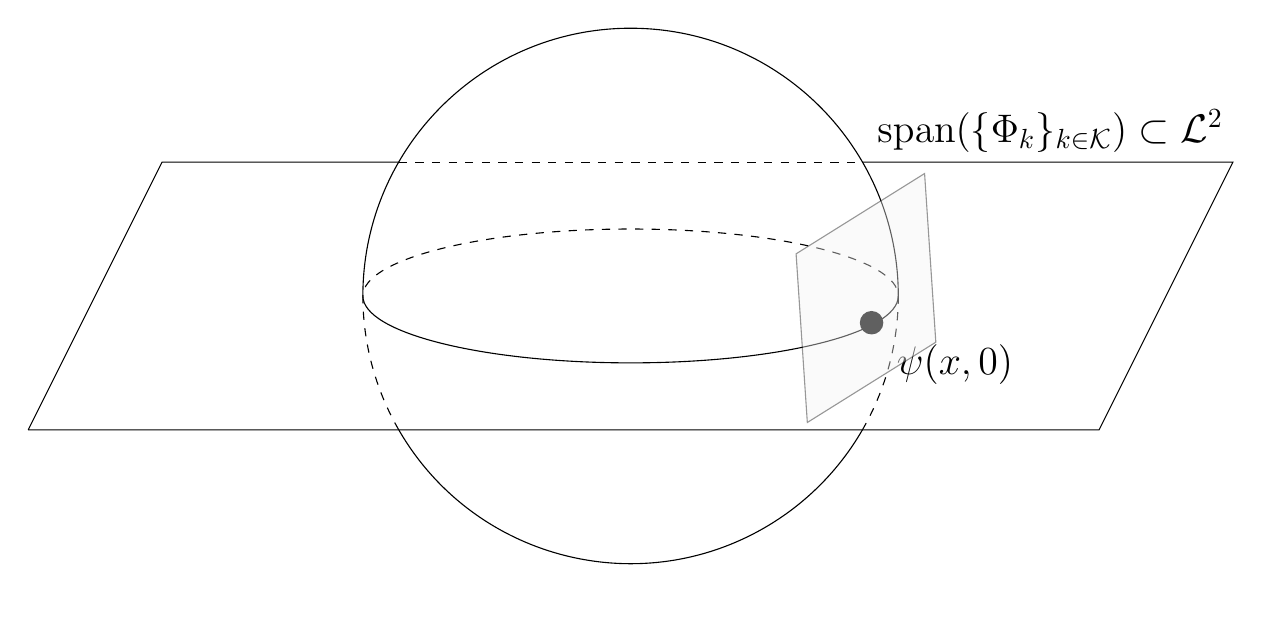
\begin{tikzpicture}[scale=1.7]
  \centering
  \coordinate (A) at (1.8,-0.2);
  \coordinate (P) at (1.5,1.1);

  \draw (0:2cm)   arc[radius=2cm,start angle=0,end angle=180]
        (210:2cm) arc[radius=2cm,start angle=210,end angle=330];
  \draw (180:2cm) arc[x radius=2cm, y radius=0.5cm, start angle=180,end angle=360];

  \draw [dashed] (210:2cm)
        arc[start angle=210,delta angle=-30,radius=2cm]
        arc[start angle=180,delta angle=-180,x radius=2cm,y radius=0.5cm]
        arc[start angle=0,delta angle=-30,radius=2cm];

  %\draw [dashed] (80:2cm and 0.5cm) -- (260:2cm and 0.5cm);
  \draw [dashed] (150:2cm) coordinate(ul) -- (30:2cm) coordinate(ur);

  \draw (-4.5,-1) -- (3.5,-1) -- (4.5,1) node[anchor=south east] 
    {\Large $ \operatorname{span}(\{\Phi_{k}\}_{k \in \mathcal{K}}) \subset \mathcal{L}^2$} -- (ur) (ul) -- (-3.5,1) -- (-4.5,-1);

  %\draw [dashed] (A) -- (P) coordinate[pos=0.47](B);
  \path (A) node[circle, fill, inner sep=3pt, label=below:{\hspace{2cm} \Large$ \psi(x,0) $}]{};
  %\path (B) node[circle, fill, inner sep=1pt, label=left:{\scriptsize$ (\xi,\eta,\zeta) $}]{};
  %\path (P) node[circle, fill, inner sep=2pt, label=above:{ }]{};
  \def\rad{1cm}
  \begin{scope}[xslant=1.6,yslant=-0.6,yshift=30,xshift=55, scale=0.3]
\filldraw[fill=gray!10,opacity=0.4]
  (-4,1) -- (3,1) -- (3,-1) -- (-4,-1) -- cycle;
\end{scope}
  %\draw [dashed] (-2,0) -- (2,0);
%\path[use as bounding box] ([yshift=-8mm]current axis.south west) rectangle (current axis.north east);
\end{tikzpicture}
\end{center}
\textcolor{red}{Would the approximation then have necessarily smaller norm...? 
only if you do the projection and do not increment the number of basis functions}
%%%%%%%%%%%%%%%%%%%%%%%%%%%%%%%%%%%%%%%%%%%%% DIRAC FRENKEL PROJECTION %%%%%%%%%%%%%%%%%%%%%%%%%%%%%%%%%%

I suppose one would diagonalise $\bm{F}$ since it is a 
symmetric matrix and obtain a fully decoupled system. 
\textcolor{red}{So what is this Kryloc space about - see Lubich}
\\
Different choices for $\mathcal{K}$ have been investigated in
\cite{lubichQuantumClassicalMolecular2008} together with the related
computational challenges.
A numerical scheme (order...) based on the splitting method 
for solving the system of equations 
\eqref{hagedorn:hagedorn_dynamics:parameters:evolution:q} -
\eqref{hagedorn:hagedorn_dynamics:parameters:evolution:Q}
can be found in \cite{lubichQuantumClassicalMolecular2008}
while an higher order method in \cite{blanesHighOrderEfficient2020}
%%%%%%%%%%%%%%%%%%%%%%%%%%%%%%%%%%%%%%%%%%%%%%%%%%%%%%%%%%%%%%%%%%%%%%%%%%%%
%
%
%
%%%%%%%%%%%%%%%%%%%%%%%%%%%%%%%%%%%%%%%%%%%%%%%%%%%%%%%%%%%%%%%%%%%%%%%%%%%
\subsubsection{Recursive relation for the coefficient matrix (better title)}
\textcolor{red}{I need to specify this somewhere but I have chosen perhaps the 
non standard convention of conjugating the second entry which will entail having to 
put the basis vectors in the second entry when doing the projection, I think the convention 
is to conjugate the first entry - check it out}
\\
For non-quadratic potentials, the major computational effort 
arises in the computation of the (time dependent) block matrix $\bm{F}$.
Its entries are $d$-dimensional integrals which must be solved at 
each time step \textcolor{red}{Check numerical scheme}.
\textcolor{blue}{
  \textbf{Numerical integration - sampling from the Gaussian}
\begin{itemize}
  \item Surely we can recycle the sampled points at time 
    zero since we can just translate the Gaussian in the integrand
    from which we are sampling from to $\bm{q} = 0$ (and off course 
    the translation in the potential term)
  \item Since the time dependence of the integral appears in the integrand 
    only in the parameter set (for non time dependent potentials), 
    we can also morph the sampled points according to how the 
    covariance matrix evolves in time...?
  \item We still obviously need evaluation of the potential at those 
    points but as far as the sampling goes it can be done only once...?
  \item Still for the potential you could also recycle the evaluation 
    for neighbouring times?
  \item How can it be that Monte Carlo is dimension independent but QMC 
    is dimension dependent but nonetheless achieves better convergence? 
    See effective dimension in \cite{wangEffectiveDimensionQuasiMonte2003} 
\end{itemize}}
\textcolor{red}{Is there any way to comment 
on} $\frac{d}{dt}\langle \varphi_k, W \varphi_l  \rangle$ - all it is 
changing are the parameters of the wavepackets - translation in position space 
and momentum space and dilation/contraction. One could imagine recycling 
the sampled points for neighbouring times? or better if I know, how the 
integral involving the Gaussian evolves, can I say anything about the 
evolution of the higher order moments. recycling the sample points since 
you would also consider tranlating the function to zero, and then simply 
apply a linear tranformation to the sampled points to account for the 
spread of the wavepacket...? Can I not apply this on the simple resulting 
integral...? I do not think so as you would have already evaluated the integrand?
whose numerical implementation 
for this algorithm can soon get out of hand. 
\textcolor{red}{What is the best that one can hope for? How would it scale 
with the dimension...? Is Monte Carlo independent of the dimension...?
would that mean I could use the same number of points independent of the dimension?#
what if I do integration and then differentiation with Monte Carlo - is that 
justified?}
\\
\\
In \cite{bourquinNumericalAlgorithmsSemiclassical2017}
this has been addressed through (sparse) quadrature methods (what about QMC?)
whose computational complexity is still exponential in nature \textcolor{red}{?}
\textcolor{red}{But why? Is there a reason why quadrature methods would be better 
in this case and MC methods?}
\textcolor{red}{what about you solve the d-dimensional gaussian integral - 
what can you say about the derivatives for the higher order terms...?}
\\
In this section, we investigate alternative numerical and asymptotic integration 
methods which have (?) better scaling performance?complexity?. 
Further, we compute the entries of $\bm{F}$ recursively from knowledge of $\bm{F}_{00}$ 
and its "higher order moments" $\langle (\bm{x} - \bm{q}) \rangle$ alone. In other words, 
given that the Hagedorn wavepackets are polynomials of degree $k$ we have used the 
linearity of the integral to compute the each monomial where the coefficients are 
hidden in the multiplying matrices...(in quotes)
Consequently, the problem will reduce to computing $\bm{F}_{00}$ and its higher 
order moments. 
\\
\\
In what follows, $W(\bm{x})$ denotes as always the non-quadratic remainder
term of the potential matrix which we will take to be real valued.
e re-write the recursive relation as \textcolor{red}{At some 
point I will consider translating everything to the origin}
\begin{equation}
  \left(\sqrt{k_j + 1 } 
  \varphi^\epsilon_{k + \langle j \rangle} \right)_{j=1}^d&=
  \sqrt{\frac{2}{\epsilon}}\bm{Q^{-1}}
  \Big( (\bm{x} - \bm{q})_j \varphi_k^\epsilon \Big)_{j=1}^d 
  -
  \bm{Q^{-1}}\bm{\overline{Q}}
  \left(\sqrt{k_j} \varphi^\epsilon_{k - \langle j \rangle } \right)_{j=1}^d
\end{equation}
Since $k_j \geq 0 \text{ } \forall \text{ } j$, let $\bm{K}$
denote the diagonal matrix with diagonal entries 
$\bm{K}_{jj} = k_j$ for $j \in \{1,...,d\}$.
Then, multiplying each side of the equality by 
$(\bm{K} + \bm{I}_d)^{-\frac{1}{2}}$ yields 
\begin{equation}
  \begin{split}
  \left( 
  \varphi^\epsilon_{k + \langle j \rangle} \right)_{j=1}^d
  =&
  \sqrt{\frac{2}{\epsilon}}
  (\bm{K} + \bm{I}_d)^{-\frac{1}{2}}\bm{Q^{-1}}
  \Big( (\bm{x} - \bm{q})_j \varphi_k^\epsilon \Big)_{j=1}^d 
  +
  \\
  &-
  (\bm{K} + \bm{I}_d)^{-\frac{1}{2}}
  \bm{Q^{-1}}\bm{\overline{Q}}
  \bm{K}^{\frac{1}{2}}
  \left( \varphi^\epsilon_{k - \langle j \rangle } \right)_{j=1}^d
  \end{split}
\end{equation}
Letting $\bm{A} = \sqrt{\frac{2}{\epsilon}}
(\bm{K} + \bm{I}_d)^{-\frac{1}{2}}\bm{Q}^{-1},
\bm{B} = (\bm{K} + \bm{I}_d)^{-\frac{1}{2}}
          \bm{Q}^{-1}\overline{\bm{Q}}
          \bm{K}^{\frac{1}{2}}$
we can re-write the above expression more coincisely as
\begin{equation}
  \begin{split}
    \Big(\varphi^\epsilon_{k + \langle j \rangle}\Big)_{j=1}^d
    =
    \bm{A} \Big( 
      (\bm{x} - \bm{q})_{j}\varphi^\epsilon_k
    \Big)_{j=1}^d
    - \bm{B} \Big(
      \varphi^\epsilon_{k - \langle j  \rangle}
      \Big)_{j=1}^d
  \end{split}
  \label{hag:dynamics:recurrence:relation:neat}
\end{equation}
Multiplying both sides by $W \overline{\varphi_l}$ 
(a scalar valued function) and 
integrating over $\mathbb{R}^d$ yields 
\begin{equation}
  \begin{split}
    \Big(
    \langle 
      \varphi^\epsilon_{k + \langle j \rangle}
      , W \varphi^\epsilon_l \rangle
    \Big)_{j=1}^d
    =
    \bm{A} \Big( 
      \langle (\bm{x} - \bm{q})_{j}\varphi^\epsilon_k
     , W \varphi^\epsilon_l \rangle
    \Big)_{j=1}^d
    - \bm{B} \Big(
      \langle 
      \varphi^\epsilon_{k - \langle j  \rangle}
      , W \varphi^\epsilon_l \rangle  
    \Big)_{j=1}^d
  \end{split}
  \label{hag:dynamics:recurrence:relation:inner:product}
\end{equation}
Note that in order to compute
$\langle \varphi^\epsilon_{k + \langle j \rangle}, W \varphi^\epsilon_l  \rangle$ 
we need the higher order moment of the previous Hagedorn wavepacket
$\langle (\bm{x} - \bm{q})_j \varphi^\epsilon_{k}, W \varphi^\epsilon_l \rangle $.
Similarly, we can derive a recurrence relation for these higher order terms.
By defining the diagonal matrix $\bm{Y}$ 
with entries $\bm{Y}_{jj} = (\bm{x} - \bm{q})_j$
and multiplying both sides of equation 
\eqref{hag:dynamics:recurrence:relation:neat} gives 
\begin{equation}
  \begin{split}
    \bm{Y}^p\Big(\varphi^\epsilon_{k + \langle j \rangle}\Big)_{j=1}^d
    =
    \bm{Y}^p\bm{A} \Big( 
      (\bm{x} - \bm{q})_{j}\varphi^\epsilon_k
    \Big)_{j=1}^d
    - \bm{Y}^p\bm{B} \Big(
      \varphi^\epsilon_{k - \langle j  \rangle}
      \Big)_{j=1}^d
  \end{split}
\end{equation}
The diagonal matrix $\bm{Y}^p$ does not commute with 
$\bm{A}$ unless the latter is also diagonal and so we have
that the higher order moments depend on the higher order 
cross term moments
\begin{equation}
  \begin{split}
    \Big((\bm{x} - \bm{q})_j^p &
    \varphi^\epsilon_{k + \langle j \rangle}\Big)_{j=1}^d
    =
    \bm{Y}^p
    \Big(
      \sum_{i=1}^d
     \bm{A}_{j,i} 
     (\bm{x} - \bm{q})_{i}\varphi^\epsilon_k
    \Big)_{j=1}^d
    - \bm{Y}^p \Big(
      \sum_{i=1}^d
      \bm{B}_{j,i}
      \varphi^\epsilon_{k - \langle i  \rangle}
      \Big)_{j=1}^d
      \\
    &= 
    \Big(
      \sum_{i=1}^d
     \bm{A}_{j,i} 
     (\bm{x} - \bm{q})^p_j(\bm{x} - \bm{q})_{i}\varphi_k
    \Big)_{j=1}^d
    - \Big(
      \sum_{i=1}^d
      \bm{B}_{j,i}
      (\bm{x}-\bm{q})_j^p
      \varphi_{k - \langle i  \rangle}
      \Big)_{j=1}^d
  \end{split}
\end{equation}
Now, repeating the same process as before, 
multiplying by the scalar $W\overline{\varphi_l}$
on both sides and integrating over $\mathbb{R}^d$ 
yields 
\begin{equation}
  \begin{split}
    &\Big(
      \langle (\bm{x} - \bm{q})_j^p 
    \varphi_{k + \langle j \rangle},
    W \varphi_l \rangle
  \Big)_{j=1}^d
    =
    \\
      =&
    \Big(
      \sum_{i=1}^d
     \bm{A}_{j,i} 
     \langle (\bm{x} - \bm{q})^p_j(\bm{x} - \bm{q})_{i}\varphi_k, 
    W \varphi_l \rangle
    \Big)_{j=1}^d
    - \Big(
      \sum_{i=1}^d
      \bm{B}_{j,i}
      \langle 
      (\bm{x} - \bm{q})_j^p
      \varphi_{k - \langle i  \rangle}
      , W \varphi_l \rangle
      \Big)_{j=1}^d
  \end{split}
  \label{hag:dynamics:recurrence:relation:inner:product:p}
\end{equation}
which now leads to finding an additional recurrence relation 
for the cross terms/moments. 
Note that equation \eqref{hag:dynamics:recurrence:relation:inner:product}
is just equation \eqref{hag:dynamics:recurrence:relation:inner:product:p} 
with $p=0$. We can write out the general expression. Letting 
$\alpha \in \mathbb{N}^d$, we then have 
\begin{equation}
  \begin{split}
    &\left(
    \left \langle
      (\bm{x} - \bm{q})^{p}_{j}
      \prod_{s=1}^{d} (\bm{x} - \bm{q})^{\alpha_s}_{s} 
      \varphi_{k + \langle j \rangle}, W \varphi_{l}
  \right \rangle
\right)_{j=1}^d
=
\\
    &
    \hspace{2cm}
    =
    \left(
      \sum_{i=1}^d
     \bm{A}_{j,i} 
     \left \langle 
     (\bm{x} - \bm{q})^p_j
     \prod_{s=1}^{d} (\bm{x} - \bm{q})^{\alpha_s}_{s} 
     (\bm{x} - \bm{q})_{i}\varphi_k,
     W \varphi_l \right \rangle
    \right)_{j=1}^d +
    \\
    &
    \hspace{2cm}
    - \left(
      \sum_{i=1}^d
      \bm{B}_{j,i}
      \left \langle 
      (\bm{x}-\bm{q})_j^p
      \prod_{s=1}^{d} (\bm{x} - \bm{q})^{\alpha_s}_{s} 
      \varphi_{k - \langle i  \rangle}, 
      W \varphi_l \right \rangle
      \right)_{j=1}^d
\end{split}
\end{equation}
We want to make clear the dependence in the computation of $F_{ij}$ on the 
other ...terms/moments?\\\\
For a given index, what other indices do I need?
To understand this dependence it suffices to work with the indices.
\\ 
Is there an easy way I can explain this? A graph? Something else?
\textbf{Simpler case:} Let $k \in \mathbb{N}^d$ and fix $l = 0_{\mathbb{N}^d}$. 
Looking at equation bla bla 
Then the intregral with $k + \langle j \rangle$ requires computation of only 
the first term in equation ... bla bla ... since the second term 
will have been already computed since we are doing this recursively.  

\textcolor{blue}{It makes sense just by arguing as them being polynomials, also 
recall that you would have had computed already the second term}
\textcolor{red}{and then what you want to say is that for a given index $\alpha$, 
what cross terms do you need to re-compute, which ones you need to recycle and so on}
\textcolor{blue}{I am 100\% sure there is a way to work through it in terms 
of indices alone...}
\textcolor{red}{I wonder if we can think of the algorithm just in terms of indeces then}
Note that we have kept $l$ fixed above, the reason being that 
we can use the conjugate symmetry property to fill in the 
other entries.
This is to be argued better but ultimately, it should be 
clear that we can construct the block matrix $\bm{F}$ from 
knowledge of $\bm{F}_{00}$ and its higher order terms alone.
\end{document}
